\section{Introduction}

Relational database has been a research hotspot for a long time, and the related achievements have already been applied in various scenarios such as finance, healthcare, and online services.
In order to manage data in relational databases conveniently and efficiently, Structured Query Language (abbr.~SQL) is presented.
Various relational database management systems implement their own version of SQL.

Recently, unstructured data become more common and the relationships between data are given importance.
Specifically, more graph-related analysis are in demand, such as neighborhood querying, reachability query, and pattern matching.
Such analysis is important in real-world applications like fraud detection and team formation, and to support such analysis efficiently, traversal on the relationships need to be sipported efficiently.
Therefore, graph databases emerges, which model data and relationships among them as graphs and build indices to accelerate graph queries.

Since relational databases and graph databases are suitable for different scenarios, an ideal situation would be to combine them.
Then, the primary task is to design a language that can express both relational and graph queries.
The striking SQL/Property Graph Queries (abbr.~SQL/PGQ) perfectly satisfies this requirement.
In detail, SQL/PGQ is a part of SQL 2023, and it has endowed traditional SQL with the ability to define and query graphs on top of relational databases.
Then, relational database management systems that implement SQL/PGQ also have the benefits from the graph data model.
In SQL/PGQ, graphs are presented as views, and the vertices and edges in the graphs are represented as tables.
Please note that with SQL/PGQ, graph queries and relational queries can be expressed in one statement and optimized together for a better execution plan.

An example of a SQL/PGQ query is provided in Example \ref{example:introduction:sqlpgq}.

\begin{example}
    \label{example:introduction:sqlpgq}
    In this example, three tables, i.e., \textbf{Person, Knows, Department}, are stored in the relational database.
    With SQL/PGQ, a graph view named \textbf{friendship\_graph} is created based on tables \textbf{Person} and \textbf{Knows}.
    Specifically, rows in table \textbf{Person} represent the vertices in the graph while rows in table \textbf{Knows} represent the edges.
    Besides, the department a person belonging to is stored in table \textbf{Person} as a foreign key (\textit{dept\_id}).

    Suppose we are going to find three persons satisfying: (1) They know each other; (2) Two of them belong to the Department of Computer Science.
    Then, the corresponding SQL/PGQ query is as follows:
    \begin{lstlisting}
        SELECT person1, person2, person3
        FROM Department p, GRAPH_TABLE (friendship_graph
            MATCH (p1:Person)-[:Knows]-(p2:Person)-[:Knows]-(p3:Person),
            (p1)-[:Knows]-(p3)
            COLUMNS (
                p1.name as pn1,
                p1.dept_id as dept1,
                p2.name as pn2,
                p2.dept_id as dept2,
                p3.name as pn3,
                p3.dept_id as dept3
            )
        ) f
        WHERE dept1 = p.dept_id
        AND dept2 = p.dept_id AND
        AND p.dept_name = 'Computer Science';
    \end{lstlisting}
    According to the first condition, the wanted three persons should form a triangle in \textbf{friendship\_graph}.
    It is a problem of pattern matching, and such triangles are searched for on the graph view.
    The output of the graph query is a table (named f) with three columns, i.e., person1, person2, and person3, representing the identifiers of the three persons, respectively.

    For the second condition, due to the existence of the foreign key, it is efficient to perform natural join between table f and table \textbf{Department} to obtain the ideal results.
    Please note that the results of graph queries in SQL/PGQ are still tables, and such returned tables can be exploited in relational queries.
\end{example}


%For a query expression based on SQL/PGQ, its physical plan can contain both relational operators and graph operators.

Given a query following the grammar of SQL/PGQ, query optimization is crucial for query processing, and the performance of the optimizer can significantly influence the efficiency of query processing.
To deal with such queries with both relational and graph queries, the existing optimizers are far from efficient.
Specifically, some methods translate graph queries to relational queries (e.g., Apache/Age).
These methods degrades into relational optimizers, and lose the chance of query optimization from the graph perspective.
Some other methods build graph indices and replace relational operators with graph operators that have better performance (e.g.~GrainDB).
In this way, the cost-based optimization only finds the optimal execution plan without being aware of the graph indices.
Therefore, the plan can be suboptimal after replacement.
In this paper, we are going to propose a new converged framework for query optimization of SQL/PGQ statements. 
In this framework, given a SQL/PGQ query, a converged logical plan is first generated.
Then, the relational subplan and graph subplans are optimized, where the graph indices are taken into consideration in the process of optimization.

For implementing such a optimization framework, there are mainly three challenges.


%e.g., build a graph view in main-memory (GRFusion, memory cost is large, limited optimization, only some rbo are applied for graph optimizers  or build indices on the adjacent relationships between vertices and edges (GrainDB, only replace hash join with getneighbor, only low-order statistics are used, limited improvement from the graph pserspective) to accelerate graph traversal.

\textbf{Challenge 1. Relational optimizers cannot be used to optimize graph queries directly (or with limited efficiency)}.
It is true that the vertices and edges in graphs can be represented as corresponding tables in relational databases, and the paths in the graphs can be translated into join operators in relational algebra.
However, since the relational optimizers only take the relational operators into consideration, some efficient graph operators (e.g., get edge, get vertex, get neighbors with graph indices) are ignored in the process of optimization.
Therefore, the search space is artificially reduced, the best physical plan are likely to be missed.
An intuitive idea is to replace some relational operators with graph operators after the physical plans are obtained (e.g., replace some join operators with getV/getE/getNeighbor in graph operators) to take advantage of the benefits brought about by graph operators.
Then, the obtained new plan are probabily not the optimizal plan, and the estimated costs are inaccurate.
Moreover, some efficient replacement cannot be applied w.r.t.~the obtained physical plan due to the order of joining tables representing vertices and edges.

\begin{figure*}
    \centering
    \begin{subfigure}[b]{0.4\linewidth}
        \centering
        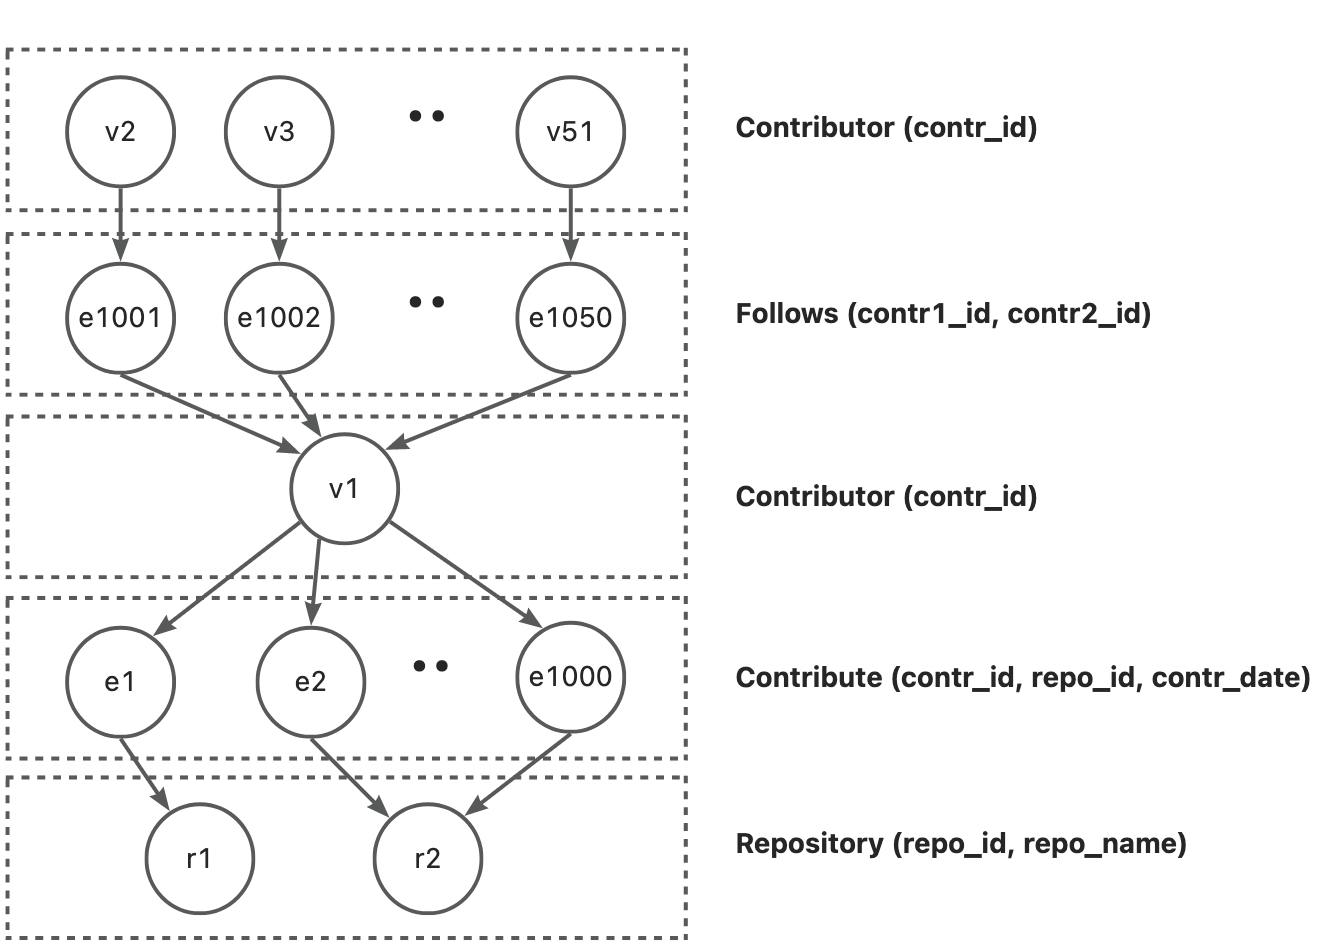
\includegraphics[width=\linewidth]{./figures/intro-order-case.png}
        \caption{Relationship 1.}
        \label{fig:intro-order-case}
    \end{subfigure}
    \begin{subfigure}[b]{0.4\linewidth}
        \centering
        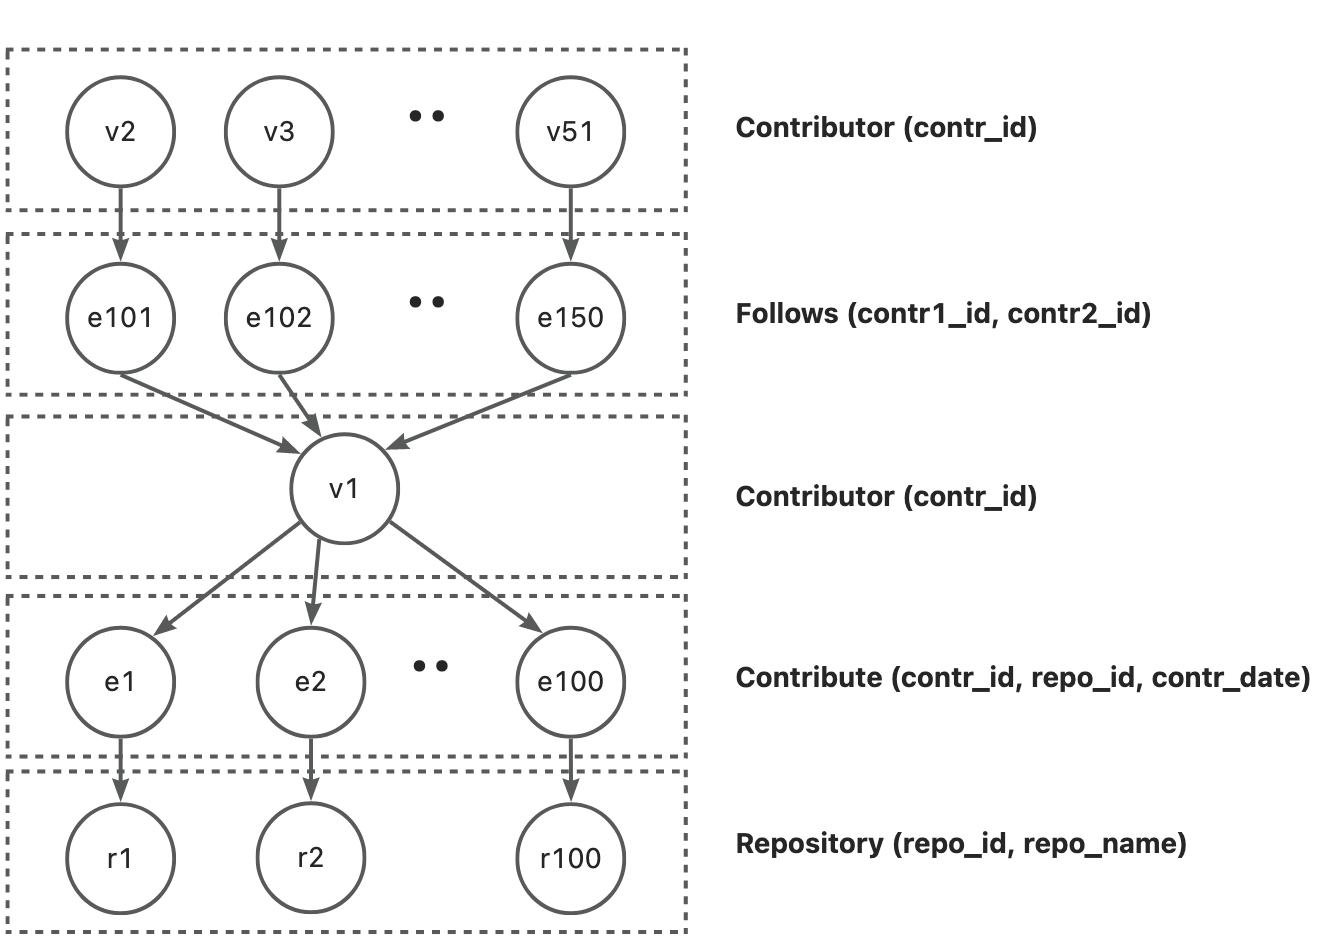
\includegraphics[width=\linewidth]{./figures/intro-order-case-2.png}
        \caption{Relationship 2.}
        \label{fig:intro-order-case2}
    \end{subfigure}
    \caption{Graphs representing the relationships among tuples in different tables. In detail, tuples in Tables \textbf{Contributor} and \textbf{Repository} represent vertices in the graph, while those in Tables \textbf{Follows} and \textbf{Contirbute} represent edges.}
    \label{fig:intro-replace-example}
\end{figure*}


\begin{example}
    Given four tables \textbf{Contributor}, \textbf{Follows}, \textbf{Contribute}, and \textbf{Repository} as shown in Fig.~\ref{fig:intro-order-case}, the relationships among their tuples are presented.
    Specifically, edge (v1, e1) means that e1.contr\_id = v1.contr\_id and edge (e1, r1) means that e1.repo\_id = r1.repo\_id.

    Given a query as follows:
    \begin{lstlisting}
        SELECT p2.contr_id, repo_name
        FROM Contributor p1, Follows f, Contributor p2, Contribute c, Repository p
        WHERE p1.contr_id = 1 
        AND p1.contr_id = f.contr2_id 
        AND p2.contr_id = f.contr1_id
        AND p1.contr_id = c.contr_id 
        AND c.repo_id = r.repo_id;
    \end{lstlisting}
    from the perspecitve of a relational database (e.g., DuckDB), the best join order can be \textbf{p1$\rightarrow$f$\rightarrow$p2$\rightarrow$c$\rightarrow$r}, since Tables \textbf{Follows} and \textbf{Contributor} has much smaller cardinalities than Table \textbf{Contribute}.
    Then, by replacing the join operators with getNeighbor, the finally obtained execution plan is \textbf{p1$\xrightarrow{\textit{getNeighbor}}$p2$\xrightarrow{\textit{getNeighbor}}$r}.

    However, as $v_1$ has much fewer neighbors in Table \textbf{Repository} than in Table \textbf{Contributor}, join order \textbf{p1$\xrightarrow{\textit{getNeighbor}}$r$\xrightarrow{\textit{getNeighbor}}$p2} would be more efficient from the perspective of graph databases.
    Therefore, it suggests that replacing relational operators with graph operators after optimization with relational optimizers can miss the optimial execution plans.

    Besides, given the relationships among the tuples as shown in Fig.~2a, the best join order from the perspective of a relational database like DuckDB can be \textbf{p1$\rightarrow$f$\rightarrow$c$\rightarrow$p2$\rightarrow$r}.
    Then, \textbf{p1$\rightarrow$f} and \textbf{c$\rightarrow$p2} cannot be replaced with \textbf{p1$\xrightarrow{\textit{getNeighbor}}$p2} and some efficient execution plans are missing.

    %An example about replace join with getV/getE/getNeighbor,
    %or the example of duckdb, whether to indicate more constraints (due to the unawareness of getNeighbor)
\end{example}


\textbf{Challenge 2. Graph optimizers are sometimes difficult to optimize relational queries directly}.
By considering relational tables as sets of vertices or edges in a graph, some relational queries can be converted to graph queries and optimized with graph optimizers. 
However, relational queries cannot always be expressed as graph queries with no effort.
For example, for relational queries with set operators (e.g., UNION, INTERSECT, or EXCEPT), it can be not straightforward to transaform them to graph queries and the obtained graph queries may be inefficient.
For another example, it is also challenging and may be inefficient to convert a relation query with subqueries to a graph query.
Moreover, GLogue is the state-of-the-art graph optimizer, and when the tables in a relational query do not forumalte a connected graph, GLogue has limited performance.

To make matters worse, translating the optimized plan back into a relational query is also very difficult.
Furthermore, the optimality of the plan may be compromised during the conversion process.
Therefore, graph optimizers are not suitable for optimizing relational queries.

A more concrete example is as follows:
\begin{example}
    Given a relational query as follows:
    \begin{lstlisting}
        SELECT p1.name, p2.name, p3.name 
        FROM Person p1, Person p2, Person p3
        WHERE p1.birthday = p2.birthday
        AND p2.birthday = p3.birthday;
    \end{lstlisting}
    This query aims to find three persons having the same birthday and only Table \textbf{Person} is involved.
    The corresponding graph query is as follows:
    \begin{lstlisting}
        MATCH (p1:Person), (p2:Person), (p3:Person)
        WHERE p1.birthday = p2.birthday
        AND p2.birthday = p3.birthday;
    \end{lstlisting}
    The graph query follows the grammar of Cypher.
    Since the graph query only consists of three isolated vertices, high-order statistics in GLogue is not utilized and the performance of GLogue is limited.

    For another example, suppose the emails of the attendees of SIGMOD 2024 and ICDE 2024 are stored in tables Att\_SIGMOD and Att\_ICDE, respectively.
    Then, the following relational query finds the common attendees of these two conferences according to persons' emails:
    \begin{lstlisting}
        SELECT email
        FROM Att_SIGMOD
        INTERSECT
        SELECT email
        FROM Att_ICDE;
    \end{lstlisting}
    The graph query following the grammar of Cypher with the same meaning might be:
    \begin{lstlisting}
        MATCH (a:Attendee)-[:ATTENDING]->(:Conference {name: 'SIGMOD 2024'})
        WITH a
        MATCH (a)-[:ATTENDING]->(:Conference {name: 'ICDE 2024'})
        RETURN a.email;
    \end{lstlisting}
    When the graph is highly connected, such a graph query can be less efficient than performing set operations on indexed tables in a relational database.
\end{example}
Moreover, relational query optimization has undergone numerous years of research and has accumulated a significant body of research findings.
Therefore, it would be unwise to abandon relational query optimization in favor of direct graph query optimization.


\textbf{Challenge 3. How to ensure worst-case-optimal joins (WCOJs)}.
Graph queries can be much more complex than relational queries, and multiple joins are common in graph queries.
Then, it is necessary to support WCOJs in the optimizer, which can reduce the complexity of 


In this paper, we propose a new converged optimization framework for SQL/PGQ.
It can optimize SQL/PGQ statements for query.
Specifically, the framework first optimize the graph queries in the statement and generate the corresponding graph physical plans.
[Since there may be join operators in the graph physical plans, the plan can be considered to be connected with join operators.
Then, the plan is combined with the left relational queries, the new query is optimized again with the relational optimizer.]

The contributions of this paper is mainly as follows:

(1) To the best of our knowledge, this is the first optimization framework for SQL/PGQ.
Property graphs are represented as views in SQL/PGQ, and vertices and edges are associated with tables in the relational databases.
Then, it is crucial to offer the converged query optimizer efficient for both relational and graph queries.

(2) The framework is the first to [unify] the inputs and outputs of the graph optimizer and relational optimizer based on the graph relational algebra, and propose the converted graph relational optimizer for SQL/PGQ queries.
In detail, given a SQL/PGQ query, it is first parsed and a converged logical plan is obtained.
This plan consists of one relational subplan and several graph subplans.
The optimizer first optimizes the graph subplans and relational subplan with graph, relational and interacting optimization strategies.

% In the framework, we design and implement numerous important operators for graph optimizer, including getV, getE, getNeighbor, and extendIntersect.
% Specifically, the extendIntersect operator is helpful in supporting worst-case optimality.

(3) Theoretical analysis on the complexity of the optimization framework is conducted.
The obtained theorems prove that for graph queries, the join order optimization with a graph optimizer can be exponentially faster than that with a relational optimizer. 
It theoretically confirms that relational optimizer is usually not suitable for graph queries, and it is indispensable for the existence of a converged optimization framework.

(4) Extensive experiments are conducted to show the efficiency of the proposed converged query optimization framework.
The experimental results show that the framework can be ?$\times$ faster than the baselines.

The rest of this paper is organized as follows.


